% Mirror: https://github.com/SIGma-UIUC/presentation-format
% --------------------------------------------------------------------
% This is a simple Beamer document that uses beamerthemesigma.sty
% Reading the comments should help you create a presentation even if
% you've never used Beamer before.
% --------------------------------------------------------------------

% Set our document class to Beamer
\documentclass[aspectratio=169, handout]{beamer}
% \documentclass[aspectratio=169, handout]{beamer}
% Add handout option to ignore pauses

% From Jeff E
\usepackage{algo}
% Some more macros
\usepackage{sigmastyle}


% Set a title
\title{A bit about Evolutionary Game Theory (EGT)}

% Set a subtitle if you desire
% \subtitle{[TAOCP 5 8.9.10.11]}

% Whoever worked on the presentation:
\author{Ahmad Abdur Rahman}

% Date looks ugly, so leave blank
\date{}

% An institute name, if you're so inclined
% \institute{University of Illinois Urbana-Champaign}

% Use the SIGma theme for this Beamer presentation
\usetheme{sigma}
% --------------------------------------------------------------------

% Begin document
\begin{document}

% Beamer calls each slide a "frame", defined within the environment:
% \begin{frame}
%   <frame content here>
% \end{frame}

% This frame is just the title.
\begin{frame}
\titlepage
\end{frame}

% A frame with the table of contents.
% This frame's title is "Outline".
% \begin{frame}{Outline}
%   \tableofcontents
% \end{frame}

% \begin{frame}{Updates!}
%   % Let's put some real content in this frame:
%   Weekly updates:
%   \begin{itemize}
%     \item SIGma is an excellent SIG.
%     \item I'm out of ideas for updates.
%   \end{itemize}
% \end{frame}

% Start a section: *sections* (subsections, etc.) are what show up in the TOC.
% \section{What is EGT?}
% % Section pages can be printed thus:
% \frame{\sectionpage}
% There's a way to automate this, see:
% https://tex.stackexchange.com/questions/178800/creating-sections-each-with-title-pages-in-beamers-slides/178803

\begin{frame}{What's game theory?}
    \begin{itemize}
        \item You may heard of game theory from \textit{A Beautiful Mind (2001)}
        \pause
        \item Maybe Nash equilibrium or The Prisoner's Dilemma
        \pause
        \item But what does the notion of 'game' imply empirically?
        \pause Simply put, game theory provides us the tools to investigate how rational agents (you or me) would want to interact in a scenario where a 'reward' is involved.
    \end{itemize}
\end{frame}

\begin{frame}
  \frametitle{Introductory notation}
  \begin{itemize} 
      \item We have set of players $N =  \{1,...,n \}$, for this presentation we're focusing on two player games.
      \pause
      \item Each player $i$ chooses an action $a_i \in A_i$ depending on past actions etc.
      \pause
      \item Each player has a respective utility function representing the 'reward' they get from the chosen move $u_i : A -> \mathbb{R}$
  \end{itemize}

  % \[
  %   \mathcal L_{\mathcal T}(\vec{\lambda})
  %   = \sum_{(\mathbf{x},\mathbf{s})\in \mathcal T}
  %      \log P(\mathbf{s}\mid\mathbf{x}) - \sum_{i=1}^m
  %      \frac{\lambda_i^2}{2\sigma^2}
  % \]
\end{frame}

% Use \pause to make stuff readable
% Large walls of text scare the audience, we don't want that
% Introducing stuff sequentially allows for questions

\begin{frame}
  % Alternate syntax for frame titles
  \frametitle{Some examples of common games}
  \begin{itemize}
      \item The two main examples of games are the Prisoner's Dilemma and the hawk-dove game (predator-prey).
      \pause 
      \item Each of the matrices below represents what's called a payoff-matrix. $V$ being anticipated value and $h$ the cost of interacting for our hawk-dove game.
  \end{itemize}
    \begin{minipage}[t]{0.50\textwidth}
        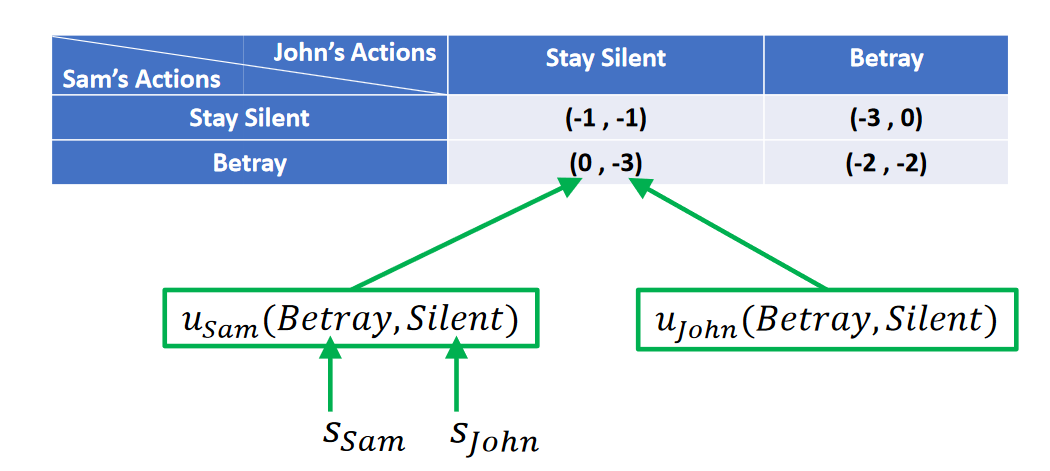
\includegraphics[width=\textwidth]{pictures/prisoners_dilemma_2.png}
    \end{minipage}
    \begin{minipage}[t]{0.45\textwidth}
        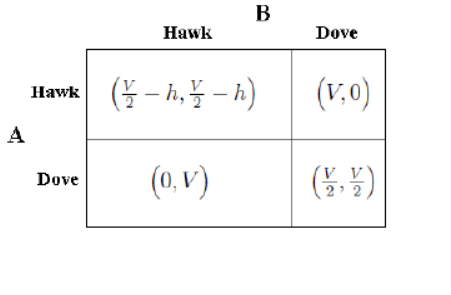
\includegraphics[width=\textwidth]{pictures/hawk_dove_payoff.png}
    \end{minipage}
\end{frame}


% However, this doesn't work in math mode. It is quite annoying to figure out
% So just copy this as reference
% This works for \onslide<> and \item<>
% Really good read on this: 
%   https://www.texdev.net/2014/01/17/the-beamer-slide-overlay-concept/
\begin{frame}{Biological contexts}
    \begin{itemize}
        \item Biologists find game theory useful in describing many natural world occurrences. It can be especially useful in approximating long-term populations.
        \pause
        \item An agent can interact in numerous ways with other agents. Each of these interaction strategies can vary depending on resulting payoffs.
        \pause 
        \item After many iterations of games, an agent would end up with a 'preferred' evolutionary stable strategy. This strategy aims to maximise the agents payoff and survival long-term.
    \end{itemize}
\end{frame}

\begin{frame}{What are the types of interactions}
    \begin{itemize}
        \item In simple contexts, you can have cooperation and combative interactions. These would 'passive' and 'aggressive' if you look at it in predator-prey terms.
        \pause 
        \item For our hawk-dove game, the hawk would end up 'winning' as it consumes doves even though the dove-dove strategy may have a higher value overall.
        \pause
        \item A cooperation strategy however can be beneficial for the prisoner's dilemma game. It turns out the best move is if both prisoners stay quiet (\textbf{no snitching!}).
    \end{itemize}    
\end{frame}

\begin{frame}{Evolutionary Stable Strategies (ESS)}
    \begin{itemize}
        \item An Evolutionary Stable Strategy (ESS) is the strategy that ends up 'dominating' long term.
        \pause
        \item An ESS would have to satisfy these two conditions
        \begin{itemize}
            \item An individual employing strategy A must do better or the same against another individual employing strategy A.
            \item Should a new strategy evolve (A') that does equally well against strategy A, for A to be an ESS, an individual employing strategy A must do better against an individual employing strategy A' than an individual employing strategy A'.
        \end{itemize}
    \end{itemize}  
\end{frame}

\begin{frame}{Further observations}
    \begin{itemize}
        \item An ESS strategy is 'pure' if it ends up as the dominant strategy and the agent doesn't diverge from that strategy.
        \pause
        \item A strategy is no longer ESS for mixed games where strategies can vary depending on relative population counts.
        \pause
        \item This is especially interesting since we see unconventional strategies dominate like 'tit-for-tat' or cooperation for minimising mutual harm. You can also have pure 'altruism' as a strategy (EA anyone?)
        \pause
        \item We can use these tools to investigate sociological instances whether it's MAD policy or some other complex group oriented interactions.
    \end{itemize}
    
\end{frame}

% \section{Conclusion}
% \frame{\sectionpage}

% Asking questions is fun but we should answer some first
\begin{frame}{}
      \begin{center}
    {\color{sigma@mainblue} \LARGE Questions?}
  \end{center}
\end{frame}

\begin{frame}{Acknowledgements}
    \begin{itemize}
        \item Material of the talk was referenced from Charles C. Cowden's \textit{Game Theory, Evolutionary Stable Strategies and the Evolution of Biological Interactions}
        % \item Olof Leimar and John M. McNamara's \textit{Game theory in biology: 50 years and onwards}
        \item CSC2556 \hyperlink{https://www.cs.toronto.edu/~nisarg/teaching/2556s21/}{Algorithms for Collective Decision Making} slides from Nisarg Shah \hyperlink{https://www.cs.toronto.edu/~nisarg/teaching/2556s21/slides/2556s21-L9.pdf}{here}
    \end{itemize}
\end{frame}

% Quotes are fun, find some to use!
\font\eightss=cmssq8
\font\eightssi=cmssqi8
\newcommand\quoteAuthorDate[3]{\begingroup
  \baselineskip 10pt
  \parfillskip 0pt
  \interlinepenalty 10000 % not needed in example
  \leftskip 0pt plus 40pc minus \parindent
  \let\rm=\eightss
  \let\sl=\eightssi
  \everypar{\sl}#1\par
  \nobreak\smallskip
  \noindent\rm--- #2\unskip\enspace(#3)\par
  \endgroup}
% If someone can figure out how to horizontally center this and make the text bigger that'd be cool
\begin{frame}
    \begin{center}
        \item \quoteAuthorDate{Playing a game is the voluntary attempt to overcome unnecessary obstacles}{Bernard Suits}{\textcolor{sigma@mainblue}{2005}}
    \end{center}
\end{frame}

% Remove this slide if you came up with all the material yourself
% \begin{frame}[allowframebreaks]{Bibliography}
%     \tiny
%     \bibliography{refs}
%     \bibliographystyle{alpha}
% \end{frame}

\end{document}